\section{Auswertung}
\label{sec:Auswertung}

\subsection{Bestimmung der maximalen magnetischen Flussdichte $|\vec{B}|_\text{max}$}

Die Messwerte der in der Probenkammer in Strahlrichtung abhängig vom Ort $z$ gemessenen magnetischen Flussdichte
$|\vec{B}(z)| = B(z)$ sind in Tabelle \ref{tab:mess1} eingetragen und in Abbildung \ref{fig:plot1} gemäß
der Vorschrift

\begin{equation}
    B(z) = a \cdot z^4 + b \cdot z^3 + c \cdot z^2 + d \cdot z + e
\end{equation}

approximiert. Dies geschieht mittels der Funktion \textit{scipy.optimize.curve\_fit} aus der Python-Bibliothek SkiPy.
$z$ ist dabei relativ von der ungefähren Probenmitte gemessen. Die negativen Werte beschreiben die Richtung zur Lichtquelle hin. 

Es ergeben sich die Approximationsparameter

\begin{align*}
    a &= \SI{-0.00953 +- 0.00026}{\milli\tesla\per\milli\meter\tothe{4}} \\
    b &= \SI{ 0.0410  +- 0.0015 }{\milli\tesla\per\milli\meter\tothe{3}} \\
    c &= \SI{-0.760   +- 0.028  }{\milli\tesla\per\milli\meter\tothe{2}} \\
    d &= \SI{ 1.74    +- 0.11   }{\milli\tesla\per\milli\meter}          \\
    e &= \SI{ 443.8   +- 0.5    }{\milli\tesla} \; .
\end{align*}

Um das Maximum der Fitkurve zu bestimmen wird die Nullstelle der ersten Ableitung

\begin{equation}
    B'(z) = \frac{\text{d}}{\text{d}z} B(z) = 4a \cdot z^3 + 3b \cdot z^2 + 2c \cdot z + d \stackrel{!}{=} 0
\end{equation}

in Abbildung \ref{fig:plot1} graphisch als $z_\text{max} = \SI{1.25}{\milli\meter}$ abgelesen und ihr die maximale magnetische Flussdichte

\begin{equation*}
    B_\text{max} = |B(z_\text{max})| = \SI{444.84}{\milli\tesla}
\end{equation*}

zugeordnet.

\begin{figure}[H]
    \centering
    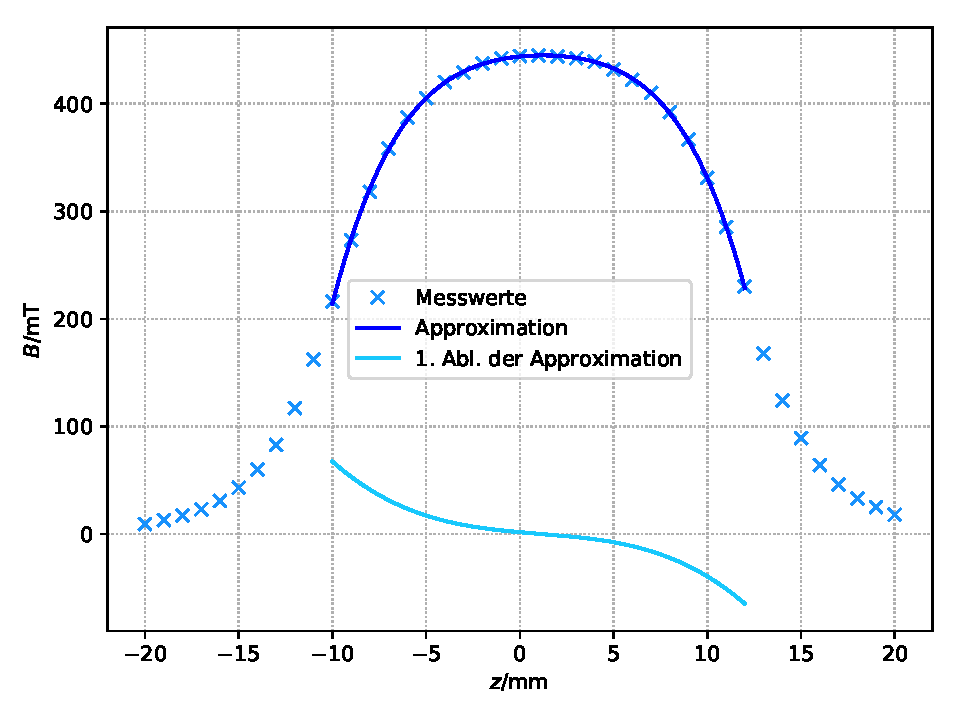
\includegraphics[scale=0.8]{content/plot1.pdf}
    \caption{Messwerte der magnetischen Feldstärke $B(z)$ in Abhängigkeit des Ortes $z$, genähert um den Hochpunkt}
    \label{fig:plot1}
\end{figure}

\begin{table}[H]
    \centering
    \caption{Messwerte magnetischen Feldstärke $B(z)$ in Abhängigkeit des Ortes $z$}
    \label{tab:mess1}
    \sisetup{table-format=2.1}
    \begin{tabular}{c c c c}
    \toprule
    $z \;/\; \si{\milli\meter}$ & $B(z) \;/\; \si{\milli\tesla}$ & $z \;/\; \si{\milli\meter}$ & $B(z) \;/\; \si{\milli\tesla}$ \\
    \midrule
        -20 &   9 &  1 & 445 \\
        -19 &  13 &  2 & 444 \\
        -18 &  17 &  3 & 442 \\
        -17 &  23 &  4 & 439 \\
        -16 &  31 &  5 & 432 \\
        -15 &  43 &  6 & 422 \\
        -14 &  60 &  7 & 410 \\
        -13 &  83 &  8 & 392 \\
        -12 & 117 &  9 & 367 \\
        -11 & 162 & 10 & 331 \\
        -10 & 216 & 11 & 285 \\
         -9 & 273 & 12 & 230 \\
         -8 & 318 & 13 & 168 \\
         -7 & 358 & 14 & 124 \\
         -6 & 387 & 15 &  89 \\
         -5 & 405 & 16 &  64 \\
         -4 & 420 & 17 &  46 \\
         -3 & 429 & 18 &  33 \\ 
         -2 & 437 & 19 &  25 \\ 
         -1 & 442 & 20 &  18 \\ 
          0 & 444 &    &     \\
    \bottomrule
    \end{tabular}
\end{table}

\subsection{Bestimmung der effektiven Masse von $\ce{GaAs}$}

Um die effektiven Massen der hochreinen und n-dotierten $\ce{GaAs}$-Proben zubestimmen, werden die in den 
Tabellen \ref{tab:mess2}, \ref{tab:mess3} und \ref{tab:mess4} aufgelisteten Daten der Faradayrotation

\begin{equation}
    \theta = \theta_1 - \theta_2
\end{equation}

mit den Probendicken $d$ normiert.
Diese betragen

\begin{align*}
    d_\text{hochrein} &= \SI{5.11}{\milli\meter} \\
    d_{N = \SI{2.8e18}{\per\cubic\centi\meter}} &= \SI{1.296}{\milli\meter} \\
    d_{N = \SI{1.2e18}{\per\cubic\centi\meter}} &= \SI{1.36}{\milli\meter} \; .
\end{align*}

Die normierte Faradayrotationen $\sfrac{\theta}{d}$ sind in Abbildung \ref{fig:plot2} gegen $\lambda^2$ aufgetragen.

Von den normierten Faradayrotationen der n-dotierten Proben werden die der hochreinen Probe abgezogen und die Differenzen
in Abbilung \ref{fig:plot3} dargestellt und linear approximiert.

Die Regressionsparameter für die Proben mit $N = \SI{2.8e18}{\per\cubic\centi\meter}$ und 
$\SI{1.2e18}{\per\cubic\centi\meter}$ ergeben sich zu:

\begin{align*}
    a_1 &= \SI{ 9.359 +- 11.1950}{\meter\tothe{-3}}\\
    b_1 &= \SI{73.905 +- 49.0425}{\meter\tothe{-1}}\\
    a_2 &= \SI{12.397 +-  9.3627}{\meter\tothe{-3}}\\
    b_2 &= \SI{ 1.424 +- 41.0156}{\meter\tothe{-1}}\; .
\end{align*}

Die effektiven Massen 

\begin{equation}
    m^* = \sqrt{\frac{e_0^3}{8\pi^2\epsilon_0 c^3} \frac{NB_\text{max}}{n} \frac{1}{a}}
\end{equation}

ergeben sich nach Umstellung der Gleichung \eqref{eqn:mass} mit einem Brechungsindex von $n = \num{3.3543}$ \cite{Brech} (S.439) zu 
 
\begin{align*}
    m^*_{1,N = \SI{2.8e18}{\per\cubic\centi\meter}} &= \num{0.10 +- 0.06} \cdot m_e \\
    m^*_{2,N = \SI{1.2e18}{\per\cubic\centi\meter}} &= \num{0.058 +- 0.022} \cdot m_e 
\end{align*}

relativ zur Elektronenmasse $m_e = \SI{9.1093837015e-31}{\kilo\gram}$.


\begin{figure}[H]
    \centering
    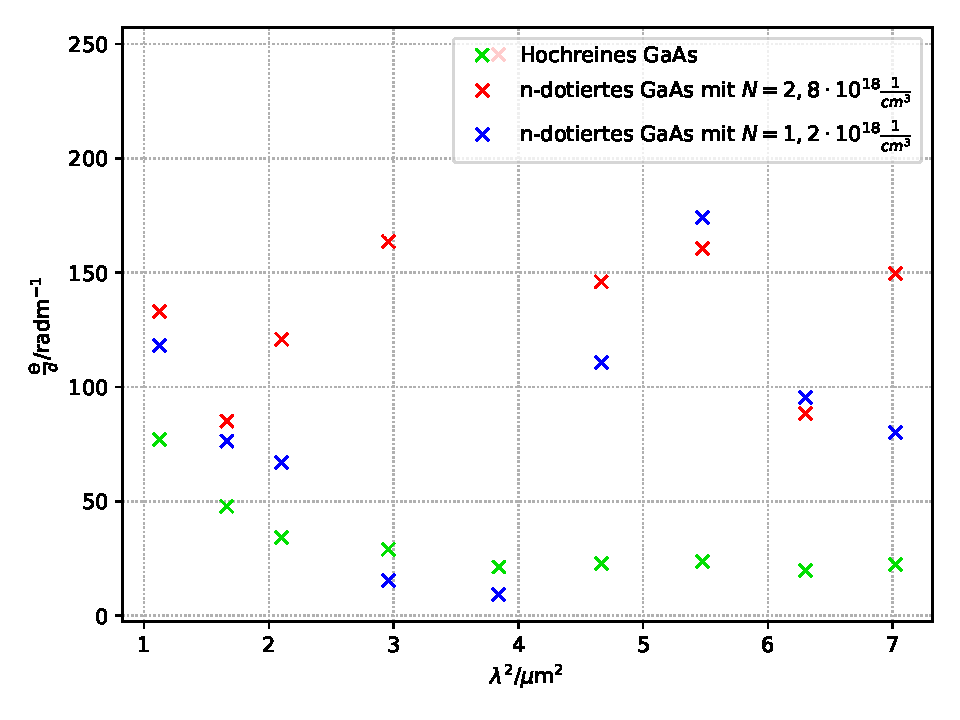
\includegraphics[scale=0.7]{content/plot2.pdf}
    \caption{Normierte Faradayrotationen $\sfrac{\theta}{d}$ der drei Proben aufgetragen gegen $\lambda^2$}
    \label{fig:plot2}
\end{figure}

\begin{table}
    \centering
    \caption{Winkelmesswerte in Abhängigkeit der gefilterten Lichtwellenlänge $\lambda$ 
        der hochreinen $\ce{GaAs}$-Probe}
    \label{tab:mess2}
    \sisetup{table-format=2.1}
    \begin{tabular}{c c c c c}
    \toprule
    $\lambda \;/\; \si{\micro\meter}$ & $\theta_1 \;/\; \si{\degree}$ &  $\theta_2 \;/\; \si{\degree}$ & 
    $\theta \;/\; \si{\radian}$ &  $\frac{\theta}{d} \;/\; \si{\radian\meter\tothe{-1}}$\\
    \midrule
        1,06 & 149,27 & 171,82 & 0,3936 & 77,02 \\
        1,29 & 151,80 & 165,78 & 0,2440 & 47,75 \\
        1,45 & 156,07 & 166,07 & 0,1745 & 34,16 \\
        1,72 & 159,30 & 167,82 & 0,1487 & 29,10 \\
        1,96 & 166,07 & 172,30 & 0,1087 & 21,28 \\
        2,16 & 173,08 & 166,40 & 0,1166 & 22,82 \\
        2,34 & 191,35 & 198,27 & 0,1208 & 23,64 \\
        2,51 & 209,03 & 203,22 & 0,1014 & 19,84 \\
        2,65 & 174,88 & 181,48 & 0,1152 & 22,54 \\
    \bottomrule
    \end{tabular}
\end{table}

\begin{table}
    \centering
    \caption{Winkelmesswerte in Abhängigkeit der gefilterten Lichtwellenlänge $\lambda$ 
        der n-dotierten $\ce{GaAs}$-Probe mit $N = \SI{2.8e18}{\per\cubic\centi\meter}$}
    \label{tab:mess3}
    \sisetup{table-format=2.1}
    \begin{tabular}{c c c c c}
    \toprule
    $\lambda \;/\; \si{\micro\meter}$ & $\theta_1 \;/\; \si{\degree}$ &  $\theta_2 \;/\; \si{\degree}$ & 
    $\theta \;/\; \si{\radian}$ &  $\frac{\theta}{d} \;/\; \si{\radian\meter\tothe{-1}}$\\
    \midrule
        1,06 & 151,78 & 161,65 & 0,1723 & 132,92 \\
        1,29 & 152,92 & 159,23 & 0,1101 &  84,98 \\
        1,45 & 152,20 & 161,18 & 0,1567 & 120,93 \\
        1,72 & 154,03 & 166,17 & 0,2119 & 163,49 \\
        1,96 & 163,05 & 181,27 & 0,3180 & 245,37 \\
        2,16 & 168,43 & 179,27 & 0,1892 & 145,98 \\
        2,34 & 190,52 & 202,45 & 0,2082 & 160,66 \\
        2,51 & 200,42 & 206,98 & 0,1145 &  88,34 \\
        2,65 & 233,22 & 244,33 & 0,1939 & 149,62 \\
    \bottomrule
    \end{tabular}
\end{table}

\begin{table}
    \centering
    \caption{Winkelmesswerte in Abhängigkeit der gefilterten Lichtwellenlänge $\lambda$ 
        der n-dotierten $\ce{GaAs}$-Probe mit $N = \SI{1.2e18}{\per\cubic\centi\meter}$}
    \label{tab:mess4}
    \sisetup{table-format=2.1}
    \begin{tabular}{c c c c c}
    \toprule
    $\lambda \;/\; \si{\micro\meter}$ & $\theta_1 \;/\; \si{\degree}$ &  $\theta_2 \;/\; \si{\degree}$ & 
    $\theta \;/\; \si{\radian}$ &  $\frac{\theta}{d} \;/\; \si{\radian\meter\tothe{-1}}$\\
    \midrule
        1,06 & 249,85 & 259,07 & 0,1609 & 118,32 \\
        1,29 & 255,23 & 261,17 & 0,1037 &  76,23 \\
        1,45 & 253,35 & 258,58 & 0,0913 &  67,12 \\
        1,72 & 253,25 & 254,45 & 0,0209 &  15,40 \\
        1,96 & 242,30 & 243,03 & 0,0127 &   9,37 \\
        2,16 & 233,95 & 242,57 & 0,1504 & 110,62 \\
        2,34 & 198,28 & 211,85 & 0,2368 & 174,15 \\
        2,51 & 202,52 & 209,95 & 0,1297 &  95,35 \\
        2,65 & 174,98 & 181,23 & 0,1091 &  80,21 \\
    \bottomrule
    \end{tabular}
\end{table}


\begin{figure}[H]
    \centering
    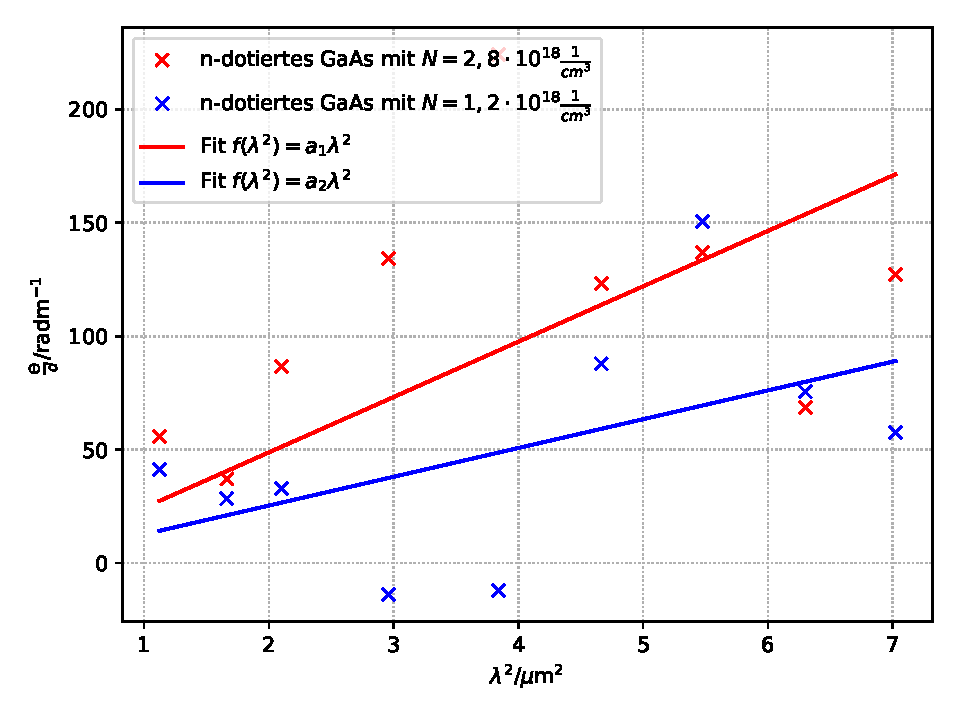
\includegraphics[scale=0.7]{content/plot3.pdf}
    \caption{Lineare Approximationen der beiden Differenzen der normierten Faradayrotation $\sfrac{\theta}{d}$ 
              der hochreinen $\ce{GaAs}$-Probe von denen der n-dotierten Proben, aufgetragen gegen $\lambda^2$}
    \label{fig:plot3}
  \end{figure}

        
        
        
        
        


  
 
  


 
 

